%% Présentation de l'entreprise et de l'endroit où vous vous situez [2-3 pages]
\section{WINDEO Green futur}
\subsection{Présentation générale}
WINDEO est un acteur européen majeur dans le domaine des énergies renouvelables. Historiquement basée sur l’éolien domestique, l’activité de Windeo s’est élargi aux produits solaires (photovoltaïque et thermique), pompes à chaleur, isolation naturelle et récupération d’eaux de pluie.\\

Premier opérateur local d'énergie verte, Windeo Green Futur agit pour le développement des énergies renouvelables et apporte des solutions accessibles aux particuliers, entreprises et collectivités locales.

\begin{figure}[!htbp]
  \centering
    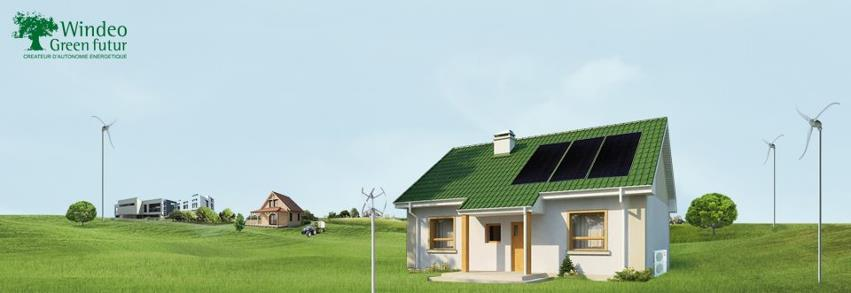
\includegraphics[width=\textwidth]{images/garde}
  \caption{Windeo Green Futur: Premier opérateur local d'énergie verte}
  %\label{fig:auth}
\end{figure}

WINDEO se distingue sur le marché des éoliennes domestique, par son savoir faire exceptionnel acquis au cours de plusieurs années de travail et d’interaction avec les principaux acteurs de cette filière.\\

Actuellement WINDEO compte 4 filiales en France et un réseau de distribution dense et en expansion. Cette forte implantation a permis l’installation de plus de 1000 turbines éoliennes de 2007 à aujourd’hui.\\

\begin{figure}[!htbp]
  \centering
    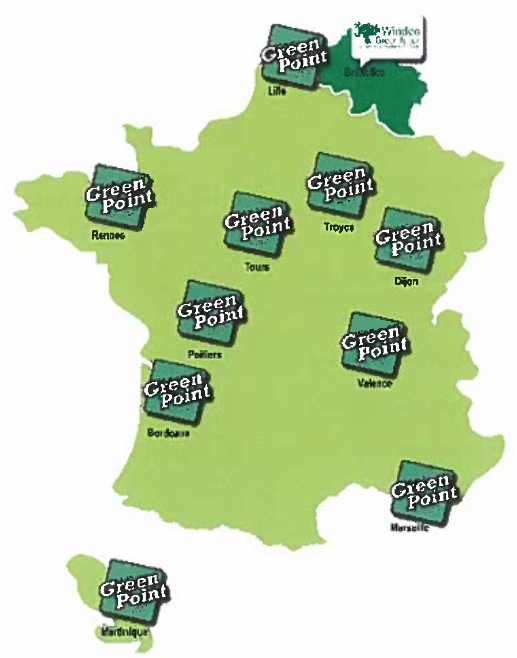
\includegraphics[scale=0.3]{images/windeo-groupe}
  \caption{Les différents points d'accueils de la société}
  %\label{fig:auth}
\end{figure}

Le concept "Green Futur", est un accompagnement dans 5 univers de ressources naturelles:\\
\begin{center}
\begin{tabular}{c l}             
  
\includegraphics[scale=0.5]{images/logo-windeo}  & \textbf{\textcolor{red}{Le Vent}}: Planète Petite éolienne \\
  
\includegraphics[scale=0.5]{images/logo-sunneo}  & \textbf{\textcolor{green}{Le Soleil}}: Le Partenaire Solaire Photovoltaïque et Thermique \\
  
\includegraphics[scale=0.5]{images/logo-watereco}  & \textbf{\textcolor{blue}{L'Eau}}: Récupérateur d'eau de pluie et traitement des eaux usées \\
  
\includegraphics[scale=0.5]{images/logo-isoleo}  & \textbf{\textcolor{cyan}{Les Matériaux naturels}}: Bois-Fibres : isolation à partir de produits naturels\\
  
\includegraphics[scale=0.5]{images/logo-aero}  & \textbf{\textcolor{magenta}{La Terre et l'air}}: Pompes à chaleur Air-Air et Air-Eau
\end{tabular}
\end{center}




\subsection{Historique de la société}

\begin{tabular}{c l}      
\textbf{2007} & Création de la société mère\\
\textbf{2008} & Lancement de l'offre Windeo\\
\textbf{2009} & Ouverture de 3 agences en France et de Windeo Liban\\
     & Lancement de l'offre commerciale SUNNEO\\
\textbf{2010} & Windeo devient le 1$^{er}$ acteur européen du petit éolien\\
     & Ouverture de 3 nouvelles agences en France \\
\textbf{2011} & Lancement de l'offre Windeo Green Futur et du concept\\
              & Green Point Déploiement du réseau de franchise
\end{tabular}
    
\subsection{Quelques chiffres concernant la société\protect\footnote{extrait du \texttt{Dossier de presse 2012} du Windeo Green Futur}}
\subsubsection{Le premier opérateur local d'énergie verte}
\begin{itemize}
\item Leader en Europe du petit éolien: plus de 1700 éoliennes vendues et près de 70\% de parts 
de marché en France en 2010
\item 2$^{eme}$ acteur sur le marché du solaire photovoltaïque en Belgique et acteur référent en 
France avec 12 MWc installés au 1$^{er}$ janvier 2012
\item 4500 clients en Europe
\end{itemize}

\subsubsection{Un groupe indépendant en croissance rapide}
\begin{itemize}
\item 100\% d'indépendance financière (5M en fonds propres)
\item 24M \euro  de chiffre d'affaires en 2011
\item 140\% de croissance du VA en un an
\item 120 collaborateurs fin 2011
\end{itemize}

\subsubsection{Une couverture internationale}
\begin{itemize}
\item 10 sites en France, 2 en Belgique et 1 au Liban
\item 6 ouvertures prévues en 2012
\item Plus de 70 distributers en Europe
\end{itemize}




\subsection{La mission de Green futur}
Windeo Green Futur développe des solutions adaptées, qu'elles soient éoliennes ou photovoltaïques, pour la production privée d'énergie renouvelable.\\

Les besoins des clients du Windeo Green Futur sont par exemple:
\begin{itemize} 
\item Effectuer des économies d’énergie / préserver l’environnement
\item Envie d’afficher son engagement écologique
\item Prévenir la hausse des couts pour l’alimentation énergétique de son ménage/
entreprise
\item Besoin d’assurer une continuité d’approvisionnement électrique (systèmes sur
batteries)
\item Curiosité vers le produit
\item etc.\\
\end{itemize}

Quotidiennement, la société relève le défi de la démocratiser et de la rendre accessible à tous en facilitant la réalisation des projets grâce à des offres clés en main et un service de proximité.\\

De par les connaissances du secteur, il est un acteur de premier plan et il doit donc devenir l'interlocuteur privilégié de leurs clients qui ne maîtrisent pas les problématiques relatives aux énergies vertes.\\

C'est pourquoi, ils les accompagnnent à tous les instants de leur projet.

\begin{figure}[!htbp]
  \centering
    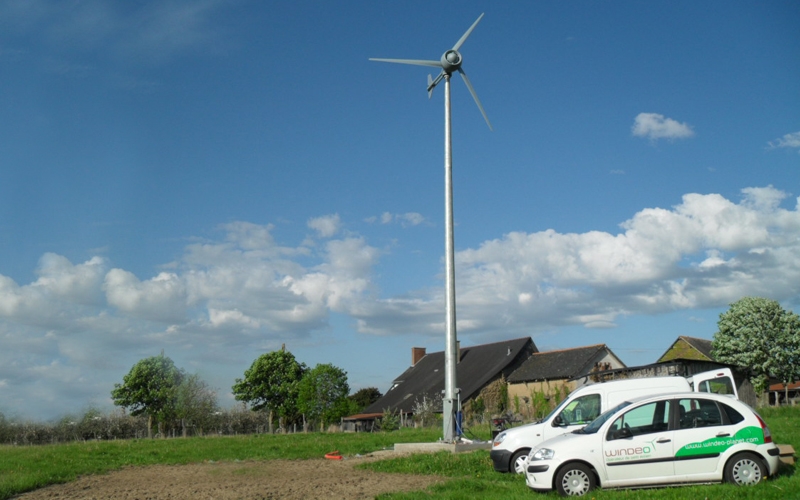
\includegraphics[width=\textwidth]{images/windeo-Evance-Domloup}
  \caption{Exemple de réalisation du Windeo}
  %\label{fig:auth}
\end{figure}

 
\section{Les differents départements}
L'équipe Windeo Green Futur est séparée en différents départements:\\

\begin{itemize}
\item Marketing
\item Centrale d’achats
\item Finance/Compta/RH
\item Pôle Ingénieurs Eolien 
\item Pôle Ingénieurs Solaire  
\item Service clients 
\item Planning \& ADV
\item Pôle technique \& SAV\\
\end{itemize}

Pour mon stage, j'ai intégré le département Pôle Ingénieurs Eolien. 
L’ensemble des équipes techniques sont supportées par ce département basé à Bruxelles.\\

Il y a 3 outils principals de communication vers le réseau exterieur et interieur 
proposé par ce département:
\begin{itemize}
\item Base de données FTP (\url{ftp.windeo-planet.com})
\item Espace intranet \url{www.windeo-planet.com/wordpress}
\item Newsletter produit mensuelle\\
\end{itemize}

L'objectif principal de mon stage est d'améliorer ces outils de communications 
pour qu'ils mieux satisfasse les exigences des clients.




